\section{Задачи на вычисление}

\paragraph{}\label{1938/194} 
\so{Теорема}.
\textbf{\emph{Во всяком треугольнике квадрат стороны, лежащей против острого угла, равен сумме квадратов двух других сторон без удвоенного произведения какой-нибудь из этих сторон на отрезок её от вершины острого угла до высоты.}}

Пусть $BC$ — сторона $\triangle ABC$ (рис.~\ref{1938/ris-203} и \ref{1938/ris-204}), лежащая против острого угла $A$, и $BD$ — высота, опущенная на сторону $AC$ (или её продолжение).
Требуется доказать, что
\[BC^2=AB^2+AC^2-2\cdot AC\cdot  AD.\]
или, обозначая длины линий малыми буквами, как указано на рисунке, надо доказать равенство:
\[a^2=b^2+c^2-2\cdot b\cdot c'\]

Из прямоугольного $\triangle BAD$ находим:
\[a^2=h^2+(a')^2.
\eqno(1)\]

Найдём каждый из квадратов $h^2$ и $(a')^2$. 
Из прямоугольного $\triangle BAD$ находим:
\[h^2=c^2-(c')^2.
\eqno(2)\]

\begin{figure}[h!]
\begin{minipage}{.48\textwidth}
\centering
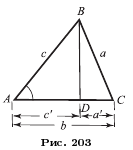
\includegraphics{mppics/ris-203}
\end{minipage}
\hfill
\begin{minipage}{.48\textwidth}
\centering
\includegraphics{mppics/ris-204}
\end{minipage}

\medskip

\begin{minipage}{.48\textwidth}
\centering
\caption{}\label{1938/ris-203}
\end{minipage}
\hfill
\begin{minipage}{.48\textwidth}
\centering
\caption{}\label{1938/ris-204}
\end{minipage}
\vskip-4mm
\end{figure}

С другой стороны, $a'=b-c'$ (рис.~\ref{1938/ris-203})) или $a'=c'-b$ (рис.~\ref{1938/ris-204}).
В обоих случаях для $(a')^2$ получаем одно и то же выражение:
\[
\begin{aligned}
(a')^2&=(b-c')^2=b^2-2\cdot a\cdot c'+(c')^2;
\\
(a')^2&=(c'-b)^2=(c')^2-2\cdot a\cdot c'+b^2.
\end{aligned}
\eqno(3)
\]

Равенство (1) можно переписать так:
\[a^2=c^2-(c')^2+b^2-2\cdot b\cdot c'+(c')^2=c^2+b^2-2\cdot b\cdot c'.\]

{\sloppy
\paragraph{}\label{1938/195}
\mbox{\so{Теорема}.}
\textbf{\emph{В тупоугольном треугольнике квадрат стороны, лежащей против тупого угла, равен сумме квадратов двух других сторон, сложенной с удвоенным произведением какой-нибудь из этих сторон на отрезок её продолжения от вершины тупого угла до высоты.}}

}



Пусть $AB$ — сторона $\triangle ABC$ (рис. \ref{1938/ris-205}), лежащая против тупого угла $C$, и $BD$ — высота, опущенная на продолжение стороны $AC$;
требуется доказать, что
\[AB^2=AC^2+BC^2+2\cdot AC \cdot  CD,\]
или, применяя сокращённые обозначения, согласно указанию на рисунке:
\[c^2=a^2+b^2+2\cdot b\cdot a'.\]

\begin{wrapfigure}{o}{45mm}
\vskip-8mm
\centering
\includegraphics{mppics/ris-205}
\caption{}\label{1938/ris-205}
\vskip0mm
\end{wrapfigure}

Из треугольников $ABD$ и $CBD$ находим:
\begin{align*}
c^2&=h^2+(c')^2=
\\
&=a^2-(a')^2+(a'+b)^2=
\\
&=a^2-(a')^2+(a')^2+2\cdot b\cdot a'+b^2=
\\
&=a^2+b^2+2\cdot b\cdot a',
\end{align*}
что и требовалось доказать.

\paragraph{}\label{1938/196}
\so{Следствие}.
Из трёх последних теорем выводим, что \emph{квадрат стороны треугольника равен, меньше или больше суммы квадратов двух других сторон, смотря по тому, будет ли противолежащий угол прямой, острый или тупой.}
Отсюда следует обратное предложение:
\emph{угол треугольника окажется прямым, острым или тупым, смотря по тому, будет ли квадрат противолежащей этому углу стороны равен, меньше или больше суммы квадратов двух других сторон.}

\paragraph{}\label{1938/197}
\so{Теорема}.
\textbf{\emph{Сумма квадратов диагоналей параллелограмма равна сумме квадратов его сторон}} (рис.~\ref{1938/ris-206}).

\begin{wrapfigure}{O}{48mm}
\centering
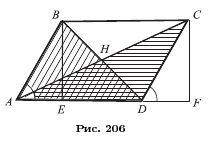
\includegraphics{mppics/ris-206}
\caption{}\label{1938/ris-206}
\end{wrapfigure}

Из вершин $B$ и $C$ параллелограмма $ABCD$ опустим на основание $AB$ перпендикуляры $BE$ и $CF$.
Тогда из треугольников $ABD$ и $ACD$ находим:
\[BD^2=AB^2+AD^2-2\cdot AD\cdot AE\]
\[AC^2=AD^2+CD^2+2\cdot AD\cdot  DF.\]

Прямоугольные треугольники $ABE$ и $DCF$ равны, так как они имеют по равной гипотенузе и равному острому углу;
поэтому $AE=DF$.
Заметив это, сложим почленно два выведенных выше равенства;
тогда $2AD\cdot  AE$ и $2AD\cdot  DF$ взаимно уничтожаются, и мы получим:
\begin{align*}
BD^2+AC^2&=AB^2+AD^2+AD^2+CD^2=
\\
&=AB^2+BC^2+CD^2+AD^2.
\end{align*}

\paragraph{Вычисление медианы треугольника.}\label{1914/241}
Медиана треугольника обыкновенно обозначается буквой $m$ (от латинского слова \emph{mediāna} — средняя), сопровождаемою (внизу) одною из маленьких букв $a$, $b$ или $c$ в зависимости от стороны треугольника, к которой проведена обозначаемая медиана.

\begin{wrapfigure}{r}{35mm}
\centering
\includegraphics{mppics/ris-1914-221}
\caption{}\label{1914/ris-221}
\end{wrapfigure}

Определим длину $m_a$ медианы, проведённой к стороне $a$ (рис.~\ref{1914/ris-221}).
Для этого продолжим медиану на расстояние $DE=AD$ и соединим точку $E$ с $B$ и с~$C$.
Мы получим параллелограмм $ABEC$ (§~\ref{1938/90}).
Применив к нему теорему о сумме квадратов диагоналей (§~\ref{1938/197}), получим:
\[a^2+(2m_a)^2=2b^2+2c^2;\]
откуда: 
\[4m_c^2=2b^2+2c^2-a^2\]
и, следовательно:
\[m_a=\tfrac 12\sqrt{2b^2+2c^2-a^2}\]

Подобным же образом можем найти $m_b$ и $m_c$.

\begin{figure}[h!]
\begin{minipage}{.48\textwidth}
\centering
\includegraphics{mppics/ris-207}
\end{minipage}
\hfill
\begin{minipage}{.48\textwidth}
\centering
\includegraphics{mppics/ris-208}
\end{minipage}

\medskip

\begin{minipage}{.48\textwidth}
\centering
\caption{}\label{1938/ris-207}
\end{minipage}
\hfill
\begin{minipage}{.48\textwidth}
\centering
\caption{}\label{1938/ris-208}
\end{minipage}
\vskip-4mm
\end{figure}

\paragraph{Вычисление высот треугольника по его сторонам.}\label{1938/198}
Определим высоту $h_a$ треугольника $ABC$, опущенную на сторону $BC=a$ (рис.~\ref{1938/ris-207} и \ref{1938/ris-208}).
Обозначим отрезки стороны $a$ (продолженной в случае тупого угла $C$, рис.~\ref{1938/ris-208}) таким образом:
отрезок $BD$, прилежащий к стороне $c$, через $c'$, а отрезок $DC$, прилежащий к стороне $b$, через $b'$.
Пользуясь теоремой о квадрате стороны треугольника, лежащей против острого угла (§~\ref{1938/194}), можем написать:
\[b^2=a^2+c^2-2\cdot a\cdot c'.\]
Из этого уравнения находим отрезок $c'$:
\[c'=\frac{a^2+c^2-b^2}{2\cdot a}\]
после чего из треугольника $ABD$ определяем высоту как катет:
\[h_a=\sqrt{c^2-\left(\tfrac{a^2+c^2-b^2}{2\cdot a}\right)^2}\]
Таким же путём можно определить в зависимости от сторон треугольника длины $h_b$, и $h_c$ высот, опущенных на стороны $b$ и $c$.
